The purpose of the pump node is to serve as an actuator and activate a pump for a specified time on request of the controller. An early draft involved a 3d printed reservoir where the electronics would be incorporated. However it turned out to be inflexible and therefore only the pump mountings have been printed and the mountings are attached to a bucket. From that bucket a hose leads to the pump and further to the flower.
It was required that the pump node supports two pumps which can be activated individually. Since the ATmega itself cannot provide sufficient current to power the pumps, a relay is used for each pump. % which relay shield do we use here?
A specific protocol takes care of the reliable communication between the pump node and the controller. It has been carefully designed to avoid freezing of the node and to ensure reliable operation of the pumps.\\

\subsubsection{Actuator}
As the task of the pump node is to water flowers, it is equipped with two pumps. Alternatively solenoid valves have been considered, however pumps are easier to use and a reliable solution. The chosen peristaltic pumps require high currents around 200mA and a voltage of 12V. Therefore they cannot be powered by Arduino pins, but have to be powered from an own power source like a voltage booster or an additional power supply. We chose an external 12V power supply to power the node.
The Arduino switches two relays which in turn power the pumps. As high current is needed, the pumps are not activated concurrently, but sequentially. They typically will be active for around 30 seconds.
Figure \ref{fig:pumpnode} illustrates a pumpnode with one pump.

\begin{figure}[H]
	\begin{center}
	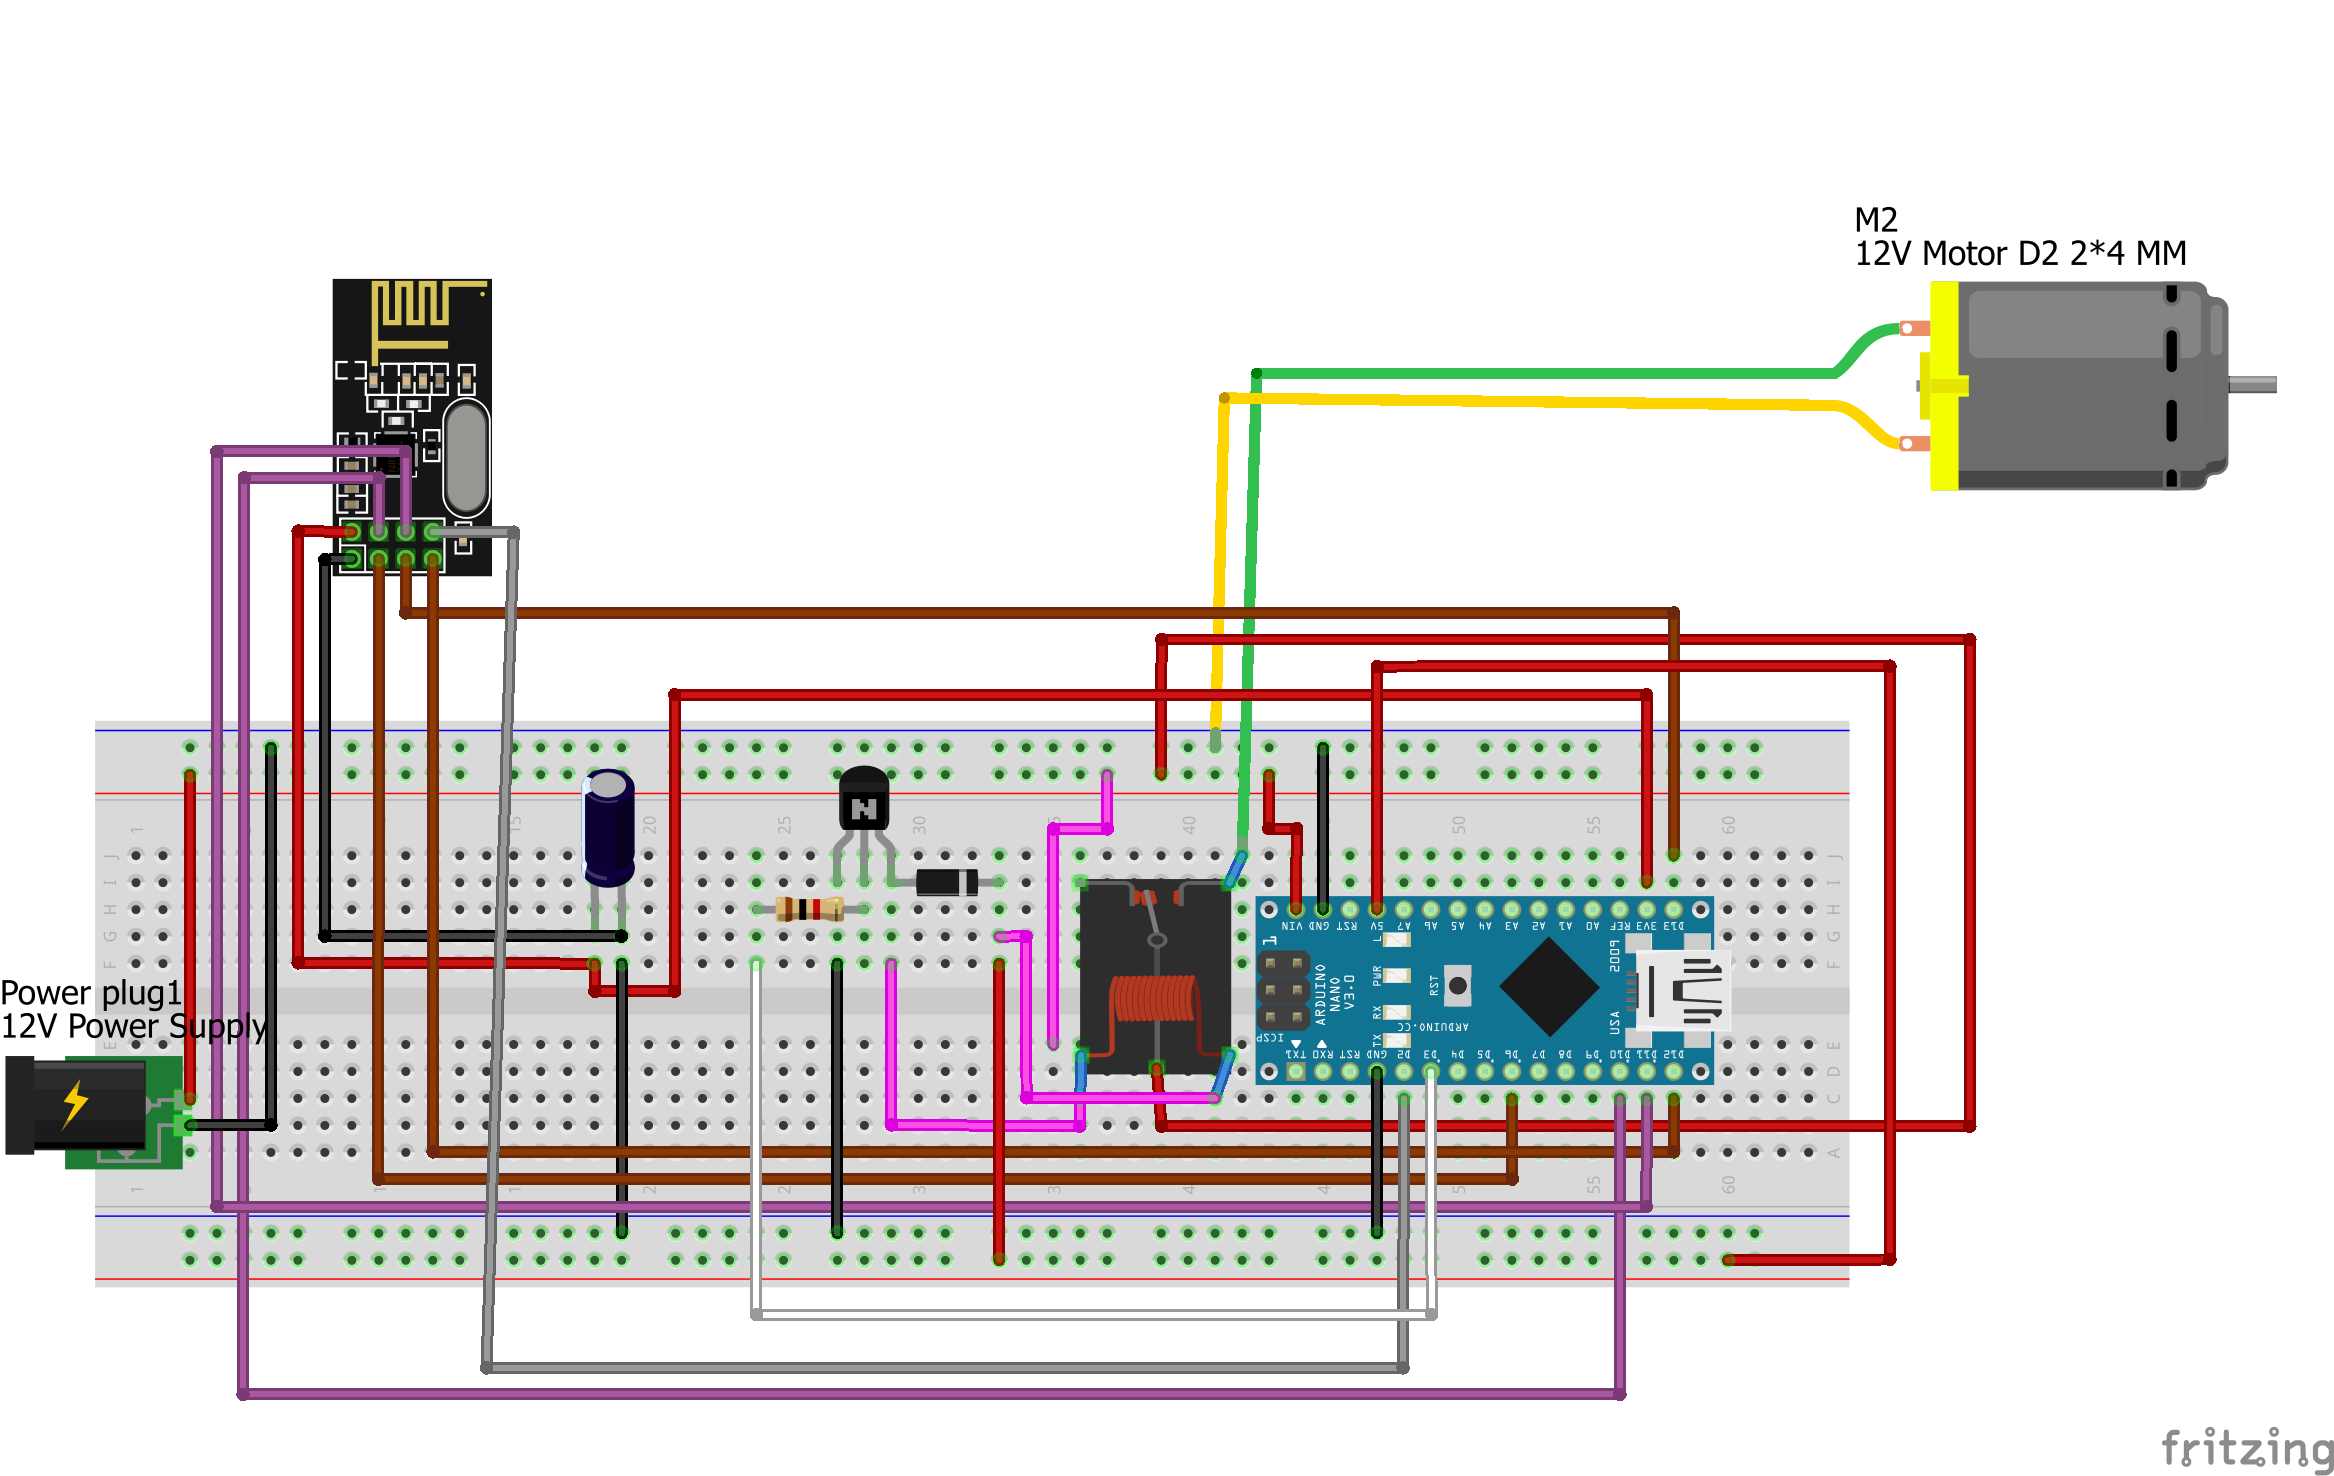
\includegraphics[scale=0.6]{images/PlantPump.png}
	\caption{Breadboard schematic of the pump node.}
	\label{fig:pumpnode}
	\end{center}
\end{figure}

\subsubsection{Fall-back Mode}
To guarantee a dependable solution resistant to external factors such as a failing internet connection or wireless jamming attacks, a fall-back mode has been implemented to water the flowers reliably, even if the control node is unavailable.

For this purpose the pump node uses all incoming messages, also those addressed to other nodes, to detect the availability of the controller. If the pump node does not receive any messages from the controller for a specified timeout\_duration, it assumes the controller is offline and goes into a fall-back mode.

The parameters for the fall-back mode are:
\begin{itemize}
\item timeout\_duration
\item enable
\item time
\item watering\_duration
\end{itemize}

These parameters can be set at the IOT front-end-interface and get transmitted to the pump nodes by the controller at the pump node registration and with every pump request. (so in case they get changed the pump node stays up to date)
In case the fall-back is disabled, no action takes place if the controller is unavailable.
In case the fall-back is enabled and the controller is unavailable, daily at the specified time the pump node pumps for the specified watering\_duration.

This mechanism does not guarantee a perfect watering, however it prevents the plants from drying.

To make the fall-back visible to the monitor node, a notification message is broadcasted via the wireless network containing the timestamp, pump duration and last timestamp from a controller message.